\documentclass[10pt]{article}

%%% These are some packages that are useful
\usepackage{amsmath,amssymb, amscd,amsbsy, amsthm, enumerate}
\usepackage[export]{adjustbox}
\usepackage{lastpage}
\usepackage[top=1in, bottom=1in, left=1in, right=1in]{geometry}
\usepackage[unicode]{hyperref}
\usepackage{tikz, pgfplots, xcolor, fancyhdr}
\usepackage{multicol}
\usepackage{lipsum}

%%% Page formatting
%\setlength{\headsep}{30pt}
\setlength{\textheight}{9in}
\newcommand{\tab}{\hspace{1cm}}
%\setlength{\parindent}{25pt}

\title{The Butterfly Effect}
\author{Antonius Torode}
\date{October 20, 2023}

%%% Header and Footer Info
\pagestyle{fancy}
\fancyhead[L]{{\large Template - \textbf{Change 03}}}
\fancyhead[C]{October 20, 2023}
\fancyhead[R]{Name: Antonius Torode}


\fancyhf{} % sets both header and footer to nothing
\renewcommand{\headrulewidth}{0pt}
% your new footer definitions here

\fancyfoot[L]{}
\fancyfoot[C]{}
\fancyfoot[R]{\thepage\ of \pageref{LastPage}}

% Used to define spacing and format of References
\let\OLDthebibliography\thebibliography
\renewcommand\thebibliography[1]{
\OLDthebibliography{#1}
\setlength{\parskip}{0pt}
\setlength{\itemsep}{0pt plus 0.3ex}
}

\newenvironment{Figure}
{\par\medskip\noindent\minipage{\linewidth}}
{\endminipage\par\medskip}


%%% Document Starts now
\begin{document}

\maketitle
\thispagestyle{fancy}

\begin{multicols}{2}

A few years back, I had a conversation with a friend about how God interacts with the physical reality that we live in. She believed that God constantly interacts, adjusts, intervenes, and monitors reality. On the contrary, I thought it was much more likely that God monitors reality consistently, but only ever needs to make small micro-adjustments. It’s probably a combination of both, but my thoughts on this come from a fundamental branch of mathematics that can be somewhat explored from a biblical perspective.

\begin{Figure}
\centering
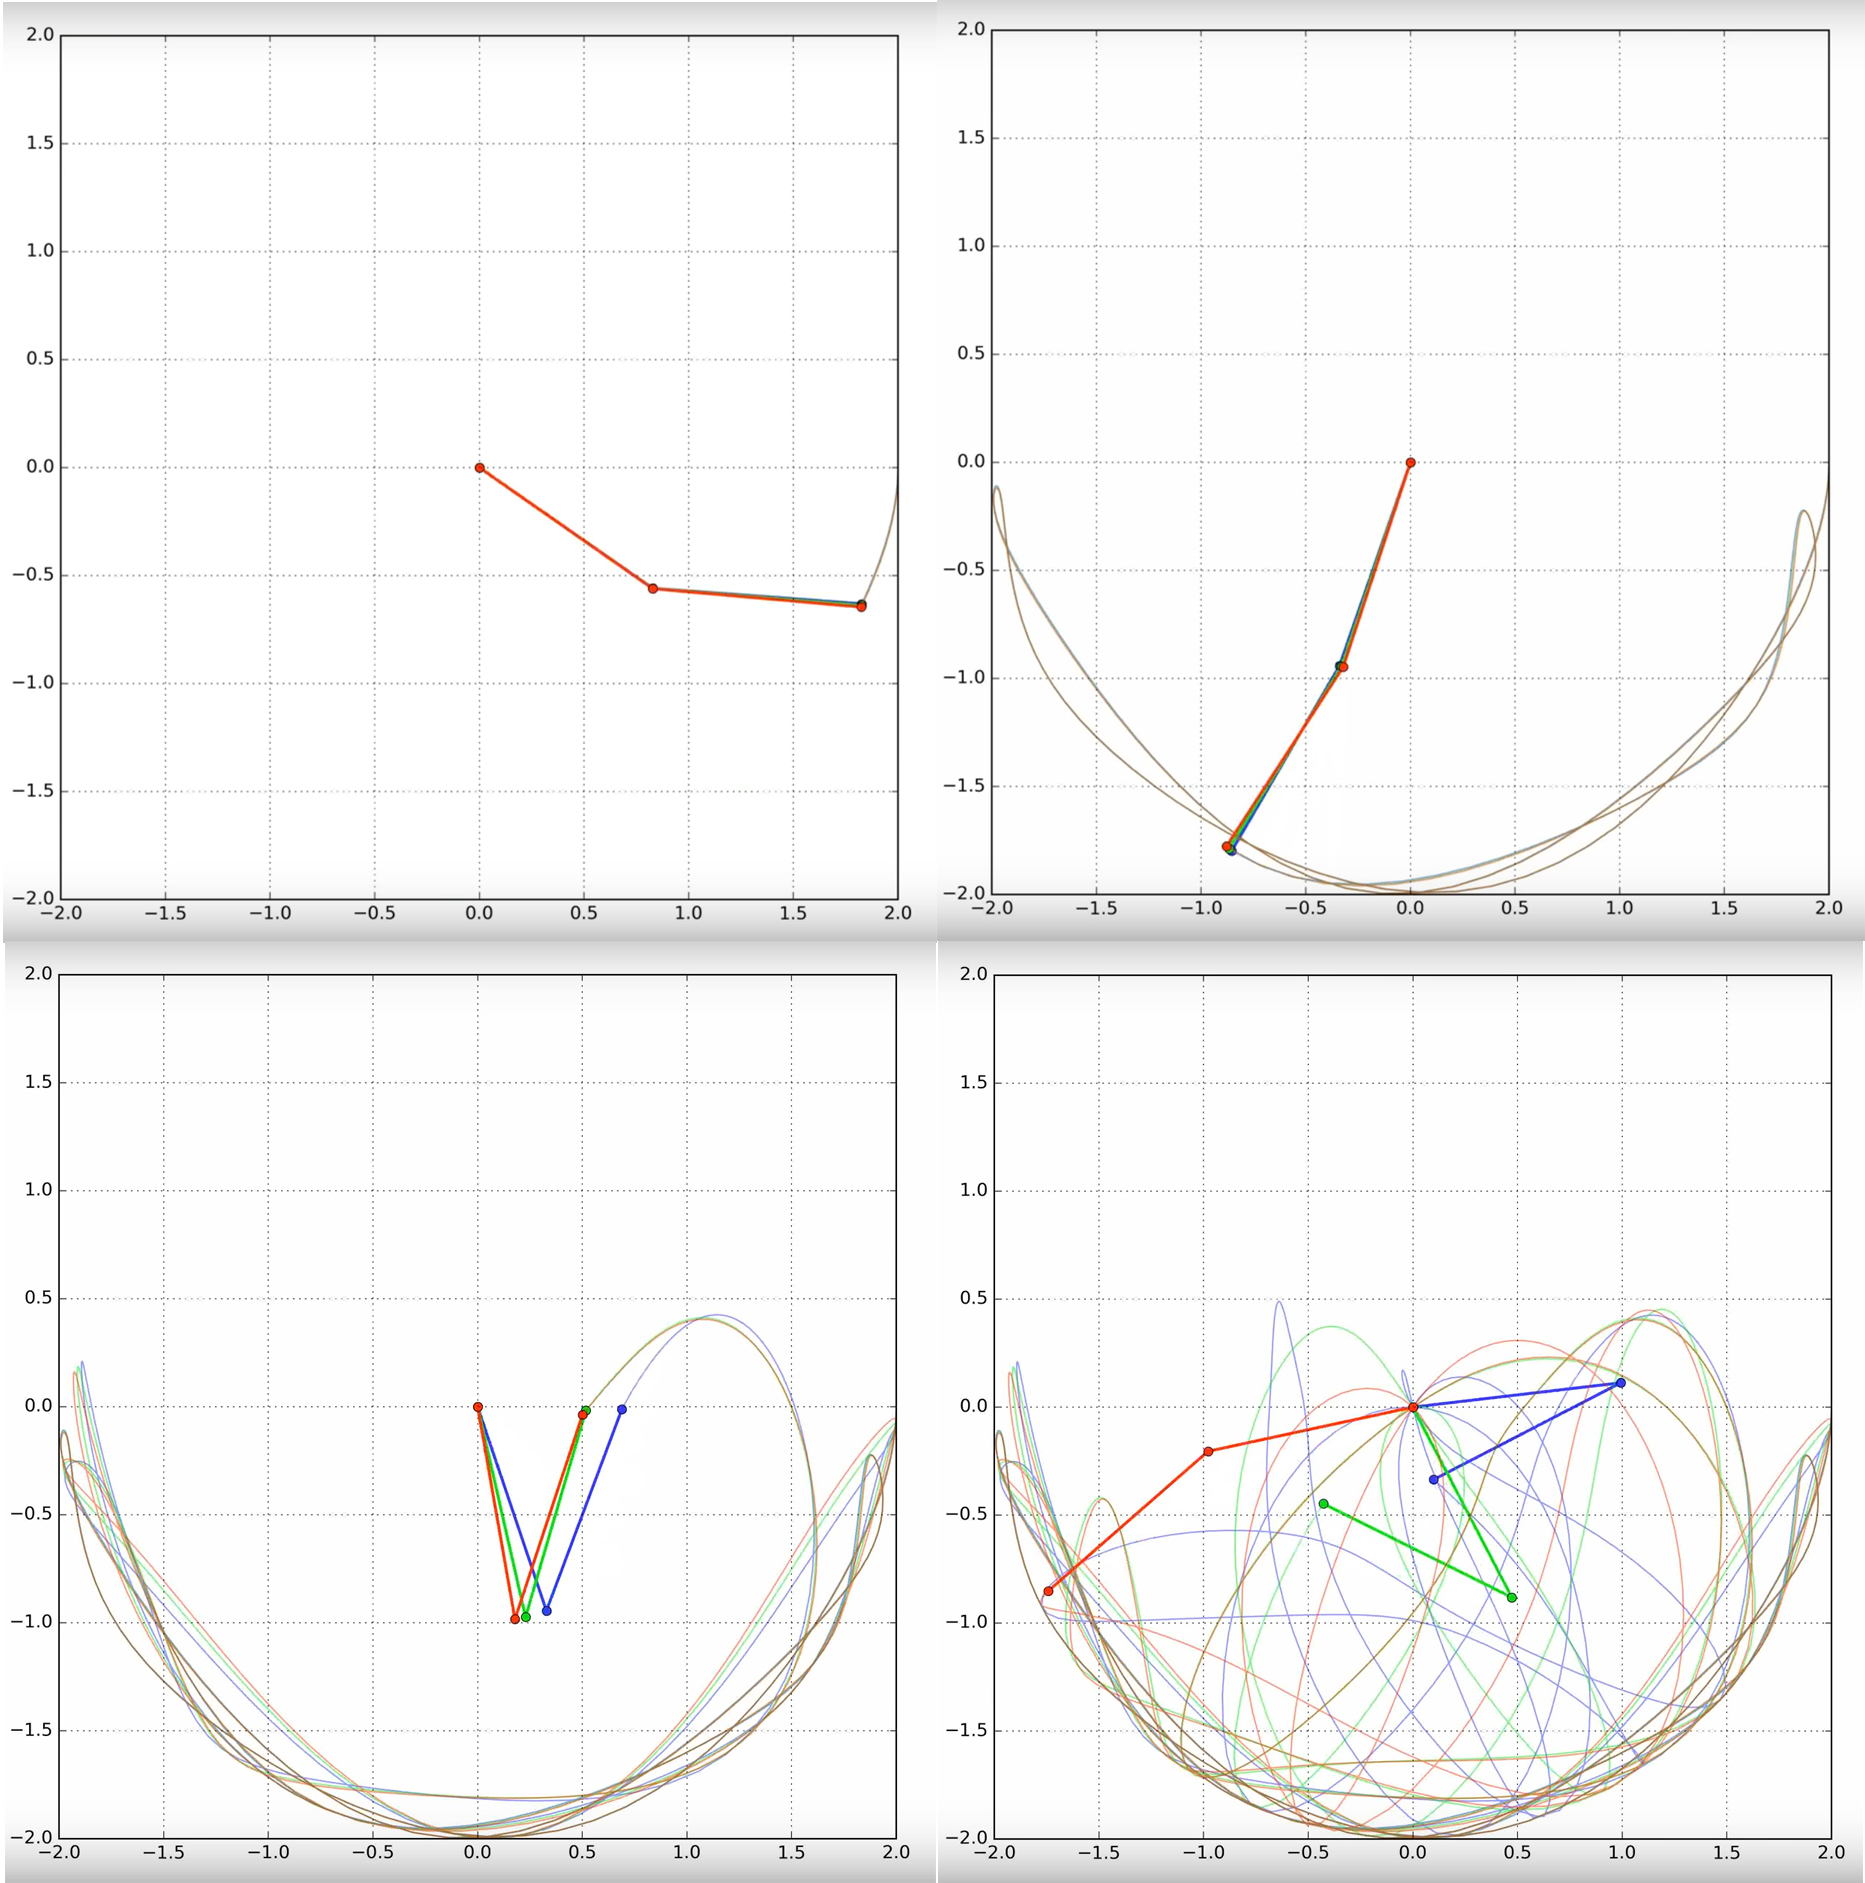
\includegraphics[width=\textwidth]{bp.jpg}
{\footnotesize Figure 1. This shows the evolution of three double pendulum paths dropped 0.5 degrees off from each other. At the start of the animation, you cannot tell there are three pendulums because they are so similar. As time progresses, they quickly diverge and become vastly different from one another. Each image is taken from the animation found from an associated video\cite{DP animation}.}
\end{Figure}

This branch of mathematics is known as chaos theory. Chaos theory has an underlying principal that many of us have probably heard of called the butterfly effect. The butterfly effect describes a scenario where a small and seemingly inconsequential change can have a large effect on something down the line. The name itself comes from the metaphorical idea that the simple flap of a butterflies wings could lead to the conditions needed in the formation of a tornado. Without that simple flap of the wings weeks earlier, the tornado may have never formed. This effect is very prevalent in physics and mathematics because many real world systems are very sensitive to small changes. One classic example is that of a double pendulum (see figure 1).

How then, does this relate to the bible? The answer is simple. Just as the flap of a butterflies wings can effect tornado weeks later. Something which is much more consequential than a butterfly flapping its wings can effect everything around us. What I'm referring to is the actions we each take. The actions each and every one of us take may seem inconsequential, but the effects they can have could easily be magnified exponentially in time. There's a wonderful example of this within the story of Joseph.

\begin{quotation}
``26. So Judah said to his brothers, “What profit is there if we kill our brother and conceal his blood? 27. Come and let us sell him to the Ishmaelites, and let not our hand be upon him, for he is our brother and our flesh.” And his brothers listened. 28. Then Midianite traders passed by; so the brothers pulled Joseph up and lifted him out of the pit, and sold him to the Ishmaelites for twenty shekels of silver. And they took Joseph to Egypt." - Genesis 37:26-28
\end{quotation}

Little did they know that this decision to sell their brother Joseph would ultimately lead to him becoming one of the most powerful people in Egypt. If this one decision was not made, none of the things that followed may have happened. His brothers had no way of knowing what future their decision would lead to. This is a perfect example for us. We often make decisions and we have no idea how they will effect us or others in the future. Because of this, we have to carefully weigh the decisions we make. It's not always possible or even easy to know what our decisions will lead to. Like with Joseph, there was no way for his brothers to know what the outcome would be.

\begin{quotation}
``8. For My thoughts are not your thoughts, Nor are your ways My ways,” says the Lord. 9. For as the heavens are higher than the earth, So are My ways higher than your ways, And My thoughts than your thoughts." Isaiah 55:8-9
\end{quotation}

What chaos theory tells us, is that in deterministic (a predictable system) systems, we can know the outcome as long as we precisely know the starting conditions and all the factors effecting that system. For mathematical pendulums, this is the case. For reality, that's not the case. Even so, with our limited human understanding we can predict and understand how things will behave and change. We cannot always do this accurately, but sometimes we are able to get extremely close. Now imagine a being so far above us in understanding, that he could know how our actions would effect reality.

\begin{quotation}
``20. But as for you, you meant evil against me; but God meant it for good, in order to bring it about as it is this day, to save many people alive." - Genesis 50:20
\end{quotation}

Just as a the flap of a butterfly's wings could metaphorically cause a tornado, our actions can cause evil or good. God knew Joseph's heart. He know how he thought and what actions he would likely take. So did God guide Joseph his whole path, or did he put him on the path and knew where it would lead? Well, there's no way of knowing for sure (and it's probably a little bit of both), but we can certainly understand how a small change can have a huge outcome.

I'd like to conclude with a personal story. About six years ago at the feast of Tabernacles in Orange beach Alabama, we received news one day that Hurricane Nate was forming to the south. This hurricane was moving faster than normal. By the time it was going to reach us in Alabama, it was predicted to be a category 3. They had began a voluntary evacuation of the area and many people were clearing out. We and many other members of the church decided to stay in town for the moment and keep a close eye on the development of the storm. The entire congregation was praying and we were waiting to see if God would intervene.

The storm had already done havoc in central America and was only in its infancy. As it began to grow over the Gulf of Mexico, everyone was getting worried. However, as we were watching the news, a drastic change began to take effect. A small vortex of cold wind began to form right in the path of the storm. When Hurricane Nate merged with this vortex, instead of continuing to grow, it began to split apart. When the storm managed to reach us in Alabama, it had lost so much of its power that it wasn't even considered a hurricane anymore. It was simple a tropical storm. The entire hurricane was thwarted by a simple vortex of cold air. When thinking about this story, it didn't seem to me like God put up a force field around us in Alabama. Rather, it seemed to me like he simply sent a little butterfly to flap its wings -- and He knew that would be enough.




\begin{thebibliography}{9}
{\footnotesize
\bibitem{DP animation} Double Pandulum Chaos Animation - https://www.youtube.com/watch?v=pEjZd-AvPco
}
\end{thebibliography}

\end{multicols}


%%%%%%%%%%%%%%%%%%%%%%%%%%%%%%%%%%%%%%%%%%%%%%%%%%%%%%%%%%%%%%%%%%%%%%%%%%%%%%%%%%%%%%%%%%%
\end{document}